Voxtral Realtime is a Transformer-based streaming ASR model that follows the stream-synchronous design of DSM. The model comprises (i) a causal audio encoder, (ii) a temporal adapter that downsamples encoder frames, and (iii) a Transformer decoder that generates text autoregressively. At each stream step, the decoder consumes a fused representation obtained by summing the current-step audio embedding with the embedding of the most recently generated text token. The overall architecture is summarized in Figure~\ref{fig:archi}, with model dimensions outlined in Table~\ref{tab:model-dims}.

\begin{figure}[t]
\centering
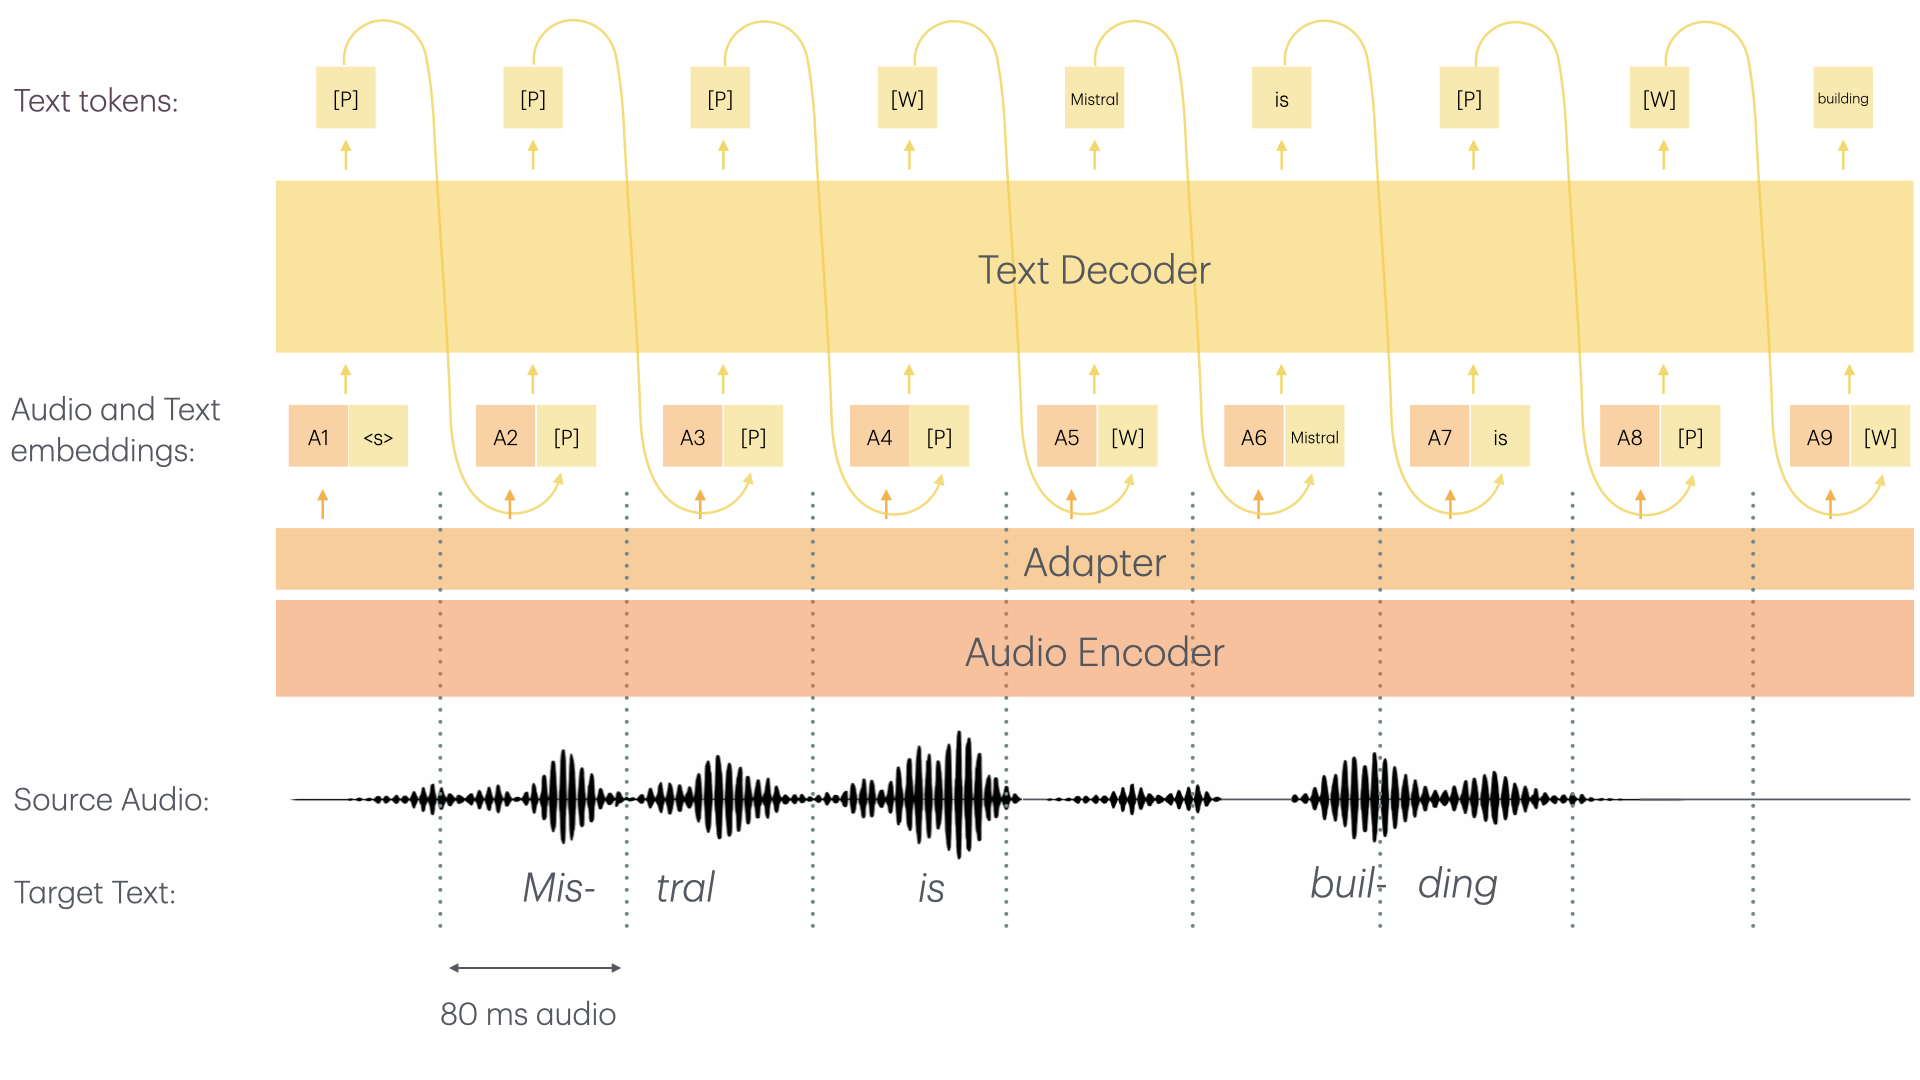
\includegraphics[width=\textwidth]{figures/streaming.004.jpeg}
\caption{
\label{fig:archi}
\textbf{Voxtral Realtime architecture and decoding scheme for a target delay $\tau=80$\,ms.} Voxtral Realtime consists of a causal audio encoder to embed the input audio stream, an MLP adapter layer to temporally downsample the audio embeddings, and a text decoder to auto-regressively generate the output text stream. The downsampled audio embeddings from the adapter and the embeddings of previously generated tokens have the same frame-rate of 12.5Hz, with each frame representing 80ms of audio. These are summed and processed by the text decoder, which predicts one token per frame. The decoder emits a padding token \texttt{[P]} while waiting for sufficient acoustic evidence. Once a word is acoustically complete and the target delay $\tau$ has elapsed, a word-boundary token \texttt{[W]} is emitted to initiate generation, followed by the corresponding subword tokens.
}
\end{figure}

\begin{table}[h]  
\centering          
\caption{
\textbf{Voxtral Realtime configuration}. For the decoder, we use grouped-query attention (GQA) \citep{ainslie2023gqa}; the number in parentheses indicates KV heads. Sliding window sizes are in frames (encoder) and tokens (decoder).
}
\label{tab:model-dims}                 
\begin{tabular}{lccccc}                   
\toprule            
\textbf{Component} & \textbf{Layers} & \textbf{Dimension} & \textbf{Heads} & \textbf{Sliding Window} & \textbf{Parameters} \\     
\midrule            
Audio Encoder & 32 & 1280 & 32 & 750 & 970M \\
Adapter MLP & 1 & 1280$\times$4 $\rightarrow$ 3072 & — & — & 25M \\
Language Decoder & 26 & 3072 & 32 (8 KV) & 8192 & 3.4B \\                  
\midrule            
\textbf{Total} & — & — & — & — & 4.4B \\     
\bottomrule         
\end{tabular}       
\end{table}

\subsection{Audio Encoder}

Audio encoders for offline ASR systems are typically trained with bidirectional attention \citep{baevski2020wav2vec20,radford2023whisper}, since the full audio signal is available. However, in real-time settings the encoder must produce representations causally, attending only to current and past inputs.

Therefore, we define a causal audio encoder architecture and train it from scratch. The waveform is converted to a log-Mel spectrogram \citep{davis1980comparison} with 128 Mel bins and a hop length of 160 samples (10\,ms at 16\,kHz). Features are processed by a causal convolutional stem with 2x temporal downsampling, followed by a stack of causal self-attention layers. The encoder emits one embedding every 20\,ms (50\,Hz).

\looseness=-1 The convolutional stem induces a finite history dependency: the output at step $t$ depends on the previous four input frames (two kernel-3 convolutions, including a strided downsampling layer). During streaming inference, we maintain a 4-frame history buffer to compute the current encoder state exactly.

\looseness=-1 In the Transformer backbone, we adopt RMSNorm, SwiGLU and RoPE—architectural choices that have been shown to improve training stability and downstream performance \citep{zhang2019rms,shazeer2020swiglu,su2023rope,touvron2023llama}. The self-attention uses a sliding window of 750 frames (15\,s at 50\,Hz) \citep{child2019sliding,beltagy2020long}, bounding memory while enabling unbounded streaming. The differences in relation to the Whisper encoder are summarized in Table~\ref{tab:archi}.

\begin{table}[t]
\centering
\caption{\textbf{Whisper vs. Voxtral Realtime encoder architectures.} Voxtral Realtime is a fully causal encoder that leverages modern architectural choices with a 750 frame sliding window.}
\label{tab:archi}
\begin{tabular}{lcccccc}
\toprule
\textbf{Model}   & \textbf{Attention} & \textbf{Norm} & \textbf{FFN} & \textbf{Pos-Enc} & \textbf{Window} & \textbf{Params (M)}      \\
\midrule
Whisper & Bidirectional & LayerNorm & GELU     & Sinusoidal  & Fixed & 640 \\
Voxtral Realtime  & Causal  & RMSNorm   & SwiGLU   & RoPE   & Sliding  & 970      \\
\bottomrule
\end{tabular}
\end{table}

\subsection{Adapter Layer}

To reduce the effective sequence length processed by the language decoder, we insert a lightweight adapter layer between the audio encoder and the decoder. This adapter consists of a single MLP that temporally downsamples the encoder outputs, reducing computational cost in the language decoder while preserving relevant acoustic information.

Following Voxtral \citep{liu2025voxtral}, we apply a downsampling factor of 4x, resulting in an effective frame rate of 12.5\,Hz. Therefore, each downsampled audio embedding represents 80\,ms of audio.

\subsection{Language Decoder} \label{sec:lang-dec}

The language decoder is a decoder-only Transformer that operates synchronously with the adapter stream, closely following the delayed-streams decoding scheme of DSM \citep{zeghidour2025streaming}. At each adapter step (80\,ms), the model performs one autoregressive decoding step. The emitted token can be either a text token or a non-emitting placeholder. The placeholder allows the model to ``wait'' when acoustic evidence is insufficient, deferring text emission until the target delay has elapsed. This mechanism enables the model to learn emission timing end-to-end, without external voice activity decection (VAD) or forced alignments. The construction of training targets is described in Section~\ref{sec:training}.

We condition the decoder on a target streaming delay $\tau$, which specifies a minimum offset between acoustic evidence and the earliest time at which corresponding text tokens may be produced, using an Adaptive RMSNorm (AdaRMSNorm) mechanism. $\tau$ is embedded as a sinusoidal embedding and projected using a small MLP with a GELU activation to a vector $g(\tau)\in\mathbb{R}^d$, where $d$ is the model dimension. This conditioning is injected additively in the normalized space on the feed-forward branch of every Transformer block; the attention branch remains unconditioned.

Specifically, given hidden states $x$, a block computes:
\[
r_{\mathrm{attn}} = \mathrm{Attn}(\mathrm{RMSNorm}(x)), \qquad h = x + r_{\mathrm{attn}},
\]
\[
r_{\mathrm{ffn}} = \mathrm{FFN}\!\left(\mathrm{RMSNorm}(h) \odot \left(1.0 + g(\tau)\right)\right), \qquad y = h + r_{\mathrm{ffn}}.
\]
% The same delay embedding is used across time steps, enabling a single model to run at multiple latency targets without changing the autoregressive factorization.
To minimize the additional parameter count, we use an inner-dimension of 32 for the MLP in $g(\tau)$, which introduces 5M extra parameters for the 4.4B model. In Section~\ref{sec:ada-rms}, we show that this form of additive conditioning is more effective than alternative time-conditioning strategies.% It's possible to further reduce the added parameters but given the negligible overhead, we leave that to future work.

The decoder uses sliding window attention with a left-context of 8192 tokens. Together with the encoder’s sliding window, this supports arbitrarily long streams with bounded memory.